\documentclass{hwz}
% \usepackage{showframe}
\usepackage{lipsum}

\begin{document}

%#############################
% Title page
%#############################
\makeTitlepage{Automatisierung von Kundenservices durch künstliche Intelligenz am Beispiel der Rückforderungseinreichung in der Krankenversicherung}{Dr. Oliver Zenklusen}{Sven Tschui}{15-522-345}{BWI-A15}{Winterthur, 2. Mai 2019}

%#############################
% Abstract
%#############################
\makeAbstract{Management Summary}{
    \lipsum[4]
}

\newpage

%#############################
% Table of contents
%#############################
\tableofcontents

\newpage

%#############################
% Declaration of authorship
%#############################
\makeDeclarationOfAuthorship{Winterthur}{2. Mai 2019}{Sven Tschui}

\newpage

%#############################
% Preface
%#############################
\makePreface{Vorwort}{
    \lipsum[3]
}

\newpage


%#############################
% Intro
%#############################
% This will add roman page numbering and page header from here on
\makeBeginMain
\section{Einleitung}

\lipsum[2]

\newpage

%#############################
% Section #1
%#############################
\section{Lorem ipsum}

\lipsum[2]

\enquote{This is a direct citation}~\autocite{Nadeau2007AClassification}. And some more text.

This is a paraphrased citation \autocite{Nadeau2007AClassification}.

\lipsum[1]

\begin{figure}[h]
\caption{Example of a parametric plot ($\sin (x), \cos(x), x$)}
\centering
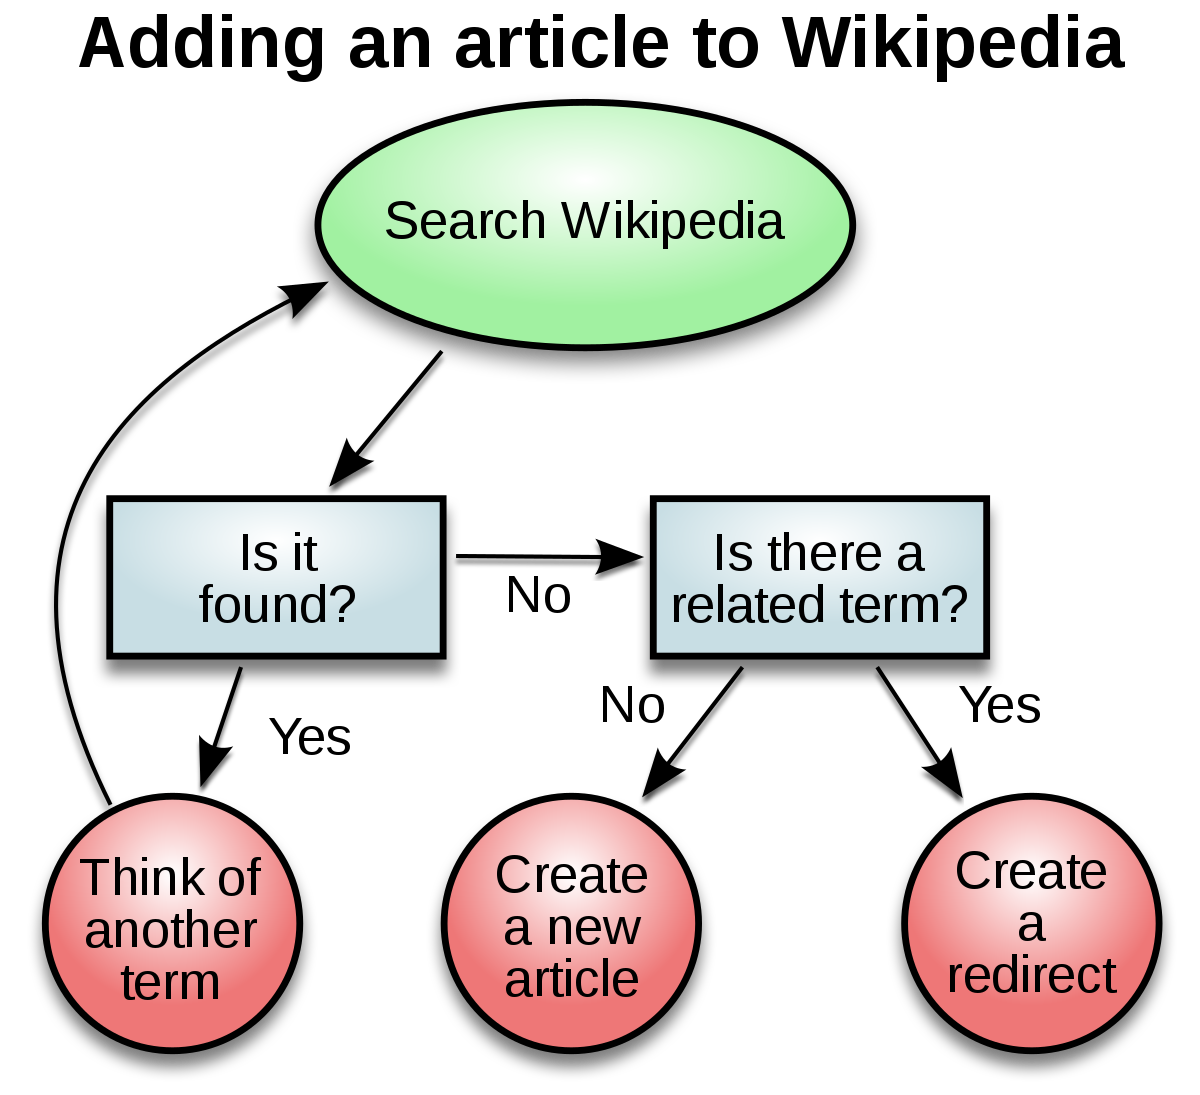
\includegraphics[width=0.5\textwidth]{graphics/wikipedia.png}
\caption*{Quelle: \textcite{BundesamtfurStatistik2018Finanzierung}}
\end{figure}

\lipsum[2]

\begin{table}[h]
\centering
\caption{Table to test captions and labels}
\label{table:1}
\begin{tabular}{||c c c c||} 
 \hline
 Col1 & Col2 & Col2 & Col3 \\ [0.5ex] 
 \hline\hline
 1 & 6 & 87837 & 787 \\ 
 2 & 7 & 78 & 5415 \\
 3 & 545 & 778 & 7507 \\
 4 & 545 & 18744 & 7560 \\
 5 & 88 & 788 & 6344 \\ [1ex] 
 \hline
\end{tabular}
\caption*{Quelle: \textcite{BundesamtfurStatistik2018Finanzierung}}
\end{table}
\newpage

%#############################
% Sub-Section #1.1
%#############################
\subsection{Sub-section Lorem ipsum}

% TODO: Text here
\lipsum[2]

\newpage

%#############################
% Section #2
%#############################
\section{Lorem ipsum 2}

% TODO: Text here
\lipsum[2]

\newpage
















\section{Notizen - Outline}

\subsection{Einleitung}
\begin{itemize}
    \item Gesundheitssystem ist grosser Kostenverursacher
    \item TG vs TP
    \begin{itemize}
         \item KVG vs. VVG
    \end{itemize}
	 \item Krankenkassen tragen mehr als 1/3 der Kosten
	 \item Grosser Verwaltungsaufwand bei den Krankenkassen
     \begin{itemize}
        \item Dadurch auch aktuelle Diskussion über Einführung Einheitskasse (relevant?)
        \item Aufzeigen der entstehenden Kosten?!
    \end{itemize}
	\item Grundversicherung stark reglementiert
    \begin{itemize}
        \item wenig Innovationsdruck/-potential
        \item Wenig Abhebung von der Konkurrenz
        \begin{itemize}
			\item Keiner macht Zusatzleistung, höchstens Abstriche (e.g. Apotheken der Assura)
        \end{itemize}
        \item Schleichender Wettbewerb
        \item Preisdifferenzierung ist enorm wichtig -> Begründung warum Forschungsfrage interessant
    \end{itemize}
	\item Digitalisierungsvorhaben des Bundes nicht erfolgreich -> Begründung warum Forschungsfrage interessant
    \begin{itemize}
        \item TARMED, SwissMedic, PatientenDossier, …
    \end{itemize}
    \item Kunde erwartet sein Geld möglichst schnell zurück
    \begin{itemize}
        \item Automatisierte verarbeitung der Rechnung erlaubt dies  -> Begründung warum Forschungsfrage interessant
    \end{itemize}
    \item Forschungsfrage
    \begin{itemize}
        \item Abgrenzung
    \end{itemize}
\end{itemize}
	
	
\subsection{Theoretischer Teil}
Was ist Machine Learning/Deep Learning?

Supervised vs Un-supervised learning?

Welche Anwendungsbereiche gibt es aktuell?

\begin{itemize}
    \item LSTM
    \begin{itemize}
        \item Einführung in Neuronale Netzwerke
        \item Was ist ein RNN/LSTM und wie funktioniert diese Art von NN
        \item Vergleich mit CNN
        \item Faktoren für den Erfolg eines NN
        \item Training
        \begin{itemize}
            \item Merkmale geeigneter Trainingsdaten
            \item Problemstellungen
            \begin{itemize}
                \item Over-fitting
            \end{itemize}
        \end{itemize}
        \end{itemize}
		\item Anwendungsgebiete für LSTM Modelle
        \begin{itemize}
	        \item OCR
            \begin{itemize}
			    \item Pre-condition für erfolgreiches OCR
                \begin{itemize}
				    \item Gute Bildqualität
                    %\begin{itemize}
					    \item Aktuell nicht gegeben
						\item Input Kanal optimieren
                        %\begin{itemize}
							\item Verbesserung des Upload Prozess des im Kundenportal
                            %\begin{itemize}
								\item Wie viele Rechnungen werden Digital eingereicht? (aktuell ca. 2/3 digital)
                            %\end{itemize}
                        %\end{itemize}
						\item Image rectification
                        %\begin{itemize}
							 \item leptonica
							 \item OpenCV
                        %\end{itemize}
                    %\end{itemize}
					\item Eine Rechnung pro Upload
                    %\begin{itemize}
						\item Aktuell nicht gegeben
						\item TARMED einfach erkennbar
                    %\end{itemize}
                \end{itemize}				
			\item Machine translation
			\item Grammatikprüfung
			\item Image recognition
        \begin{itemize}
            \item Nicht wirklich relevant für diese Arbeit
        \end{itemize}
		\item Text Classification
        \begin{itemize}
			\item Vergleich mit klassischem NLP?
			\item Warum LSTM und nicht klassisches NLP?
        \end{itemize}
        \end{itemize}
		    \item Named Entity Recognition (NER)
        \begin{itemize}
			\item Erkennung von Namen
			\item NLP vs Machine Learning basiert
        \end{itemize}
    \end{itemize}
	\item Struktur-Anforderungen der Daten für die Weiterverarbeitung
    \begin{itemize}
		\item Syrius requirements
		\item Fachliche Anforderungen
        \begin{itemize}
    		\item KVG vs. VVG beachten
        \end{itemize}
    \end{itemize}
    \item Lösungen in anderen Branchen
    \item Lösungen von anderen Unternehmen
    \begin{itemize}
		\item Man-power
        \begin{itemize}
		    \item Assura 500 / CSS 300
            \begin{itemize}
			    \item TODO: Diese Daten sind nur "Hörensagen"
            \end{itemize}
        \end{itemize}
    \end{itemize}
\end{itemize}


\subsection{Empirischer Teil}
\begin{itemize}
    \item Methodik
    \begin{itemize}
		\item Prototyping
		\item Messkriterien des Prototypen
		\item Begrüdnung des Vorgehens
    \end{itemize}
	\item Prototyp
    \begin{itemize}
		\item OCR mittels Tesseract
        \begin{itemize}
			\item Trainieren der LSTM engine mittels artificial training data aus TARMED datenbank
			\item Artificial data wird analog eingereichter Rechnungen gemacht
            \begin{itemize}
				\item Schrfitart
				\item Noise
				\item Verzerrung
            \end{itemize}
        \end{itemize}
	    \item Spell Checking mittels eigenem LSTM Modell
        \begin{itemize}
		    \item Inspiration an DeepSpell, etc.
		    \item Training des Modells anhand artificial spelling errors basierend auf
            \begin{itemize}
				\item Google Training Datasets
				\item TARMED tarifen
				\item SYR Codes
				\item EMR Methods
				\item Other Methods
				\item Custom Tarifziffern
				\item Care Providers (Names, Addresses, …)
				\item Real Invoices
				\item Medizinischen Texten / Anamnese
            \end{itemize}
        \end{itemize}
    \end{itemize}
    \item Noise reduction
    \begin{itemize}
	    \item Pre and/or Post OCR
        \item Post OCR
        \begin{itemize}
	    	\item NN with input word + confidence -> output: noise | no-noise
        \end{itemize}
    \end{itemize}
    \item Erkennung von mehreren Rechnungen in einem Upload
    \begin{itemize}
	    \item Mehrere auf einem Bild
	    \item Mehrere auf mehreren Bildern
    \end{itemize}
    \item Klassifizierung von Rechnungen
    \begin{itemize}
		\item Traditioneller Ansatz für TARMED ja/nein
		\item LSTM Text Classification für "Prosa" (non-TARMED) Rechnungen
    \end{itemize}
    \item Strukturieren von Daten
    \begin{itemize}
		\item TARMED gut strukturierbar
		\item Für andere Rechnungen wird’s etwas schwieriger
        \begin{itemize}
			\item Patienten Erkennung
			\item Care Provider Erkennung
			\item Tabellen Erkennung
            \begin{itemize}
			    \item Erkennung der einzelnen Positionen
            \end{itemize}
        \end{itemize}
        \item Business Rules zur automatisierten Verarbeitung    
    \end{itemize}  
\end{itemize}

\subsection{Schlussfolgerungen und Empfehlungen}
\begin{itemize}
	\item Bewertung des Prototypen
	\item Beantwortung der Forschungsfrage
	\item Reflexion
	\item Empfehlungen / Zukunft
  \begin{itemize}
		\item Erweitern der Pipeline für andere Rechnungstypen (e.g. Fitnessabos)
		\item Erweitern der Business Rules
		\item On-Device OCR/NER um den upload Prozess zu verbessern
    \begin{itemize}
			\item Benutzer soll den Patientennamen nicht eingeben müssen, er soll erkannt werden
			\item Benutzer kann die erhobenen Daten direkt gegenprüfen
Bspw. Behandlungsdatum, etc.
    \end{itemize}
  \end{itemize}
\end{itemize}
 
\section{Notizen - sonstiges}
 
\subsection{Lösungsansatz ``Input Pipeline''}
\begin{itemize}
    \item Erste Optimierung bereits beim Kunden, da dort ``Crowd Sourcing'' betrieben werden kann
    \begin{itemize}
        \item Image rectification mit anpassungsmöglichkeit durch Enduser (analog OfficeLens)
        \item Quality Checking
    \end{itemize}
    \item Optimierung auf der Service Seite
    \begin{itemize}
        \item Gray Scale
    \end{itemize}
    \item OCR
    \begin{itemize}
        \item LSTM basierter Ansatz
        \begin{itemize}
            \item Vergleich zur feature detection basierten vorgehensweise (Stats, warum was besser ist)
        \end{itemize}
    \end{itemize}
\end{itemize}

Machine Learning ist sehr breit
  - Text Mining
  - Deep Learning
  - OCR
  - Classification
  - Image optimization
  
\newpage













%#############################
% Appendix
%#############################
\section{Anhang}

\makeBibliography{Anhang}{Literaturverzeichnis}

\newpage

\makeListOfTablesAndFigures{Tabellen- und Abbildungsverzeichnis}

\end{document}